% Options for packages loaded elsewhere
\PassOptionsToPackage{unicode}{hyperref}
\PassOptionsToPackage{hyphens}{url}
% !TeX program = pdfLaTeX
\documentclass[12pt]{article}
\usepackage{amsmath}
\usepackage{graphicx,psfrag,epsf}
\usepackage{enumerate}
\usepackage[]{natbib}
\usepackage{textcomp}


%\pdfminorversion=4
% NOTE: To produce blinded version, replace "0" with "1" below.
\newcommand{\blind}{0}

% DON'T change margins - should be 1 inch all around.
\addtolength{\oddsidemargin}{-.5in}%
\addtolength{\evensidemargin}{-1in}%
\addtolength{\textwidth}{1in}%
\addtolength{\textheight}{1.7in}%
\addtolength{\topmargin}{-1in}%

%% load any required packages here



% tightlist command for lists without linebreak
\providecommand{\tightlist}{%
  \setlength{\itemsep}{0pt}\setlength{\parskip}{0pt}}

% From pandoc table feature
\usepackage{longtable,booktabs,array}
\usepackage{calc} % for calculating minipage widths
% Correct order of tables after \paragraph or \subparagraph
\usepackage{etoolbox}
\makeatletter
\patchcmd\longtable{\par}{\if@noskipsec\mbox{}\fi\par}{}{}
\makeatother
% Allow footnotes in longtable head/foot
\IfFileExists{footnotehyper.sty}{\usepackage{footnotehyper}}{\usepackage{footnote}}
\makesavenoteenv{longtable}



\IfFileExists{bookmark.sty}{\usepackage{bookmark}}{\usepackage{hyperref}}
\IfFileExists{xurl.sty}{\usepackage{xurl}}{} % add URL line breaks if available
\hypersetup{
  pdftitle={Maximizing Fairness with Synthetic data: Access to Emergency Fund in Sub-Saharan Africa},
  pdfkeywords={Fairness metrics; emergency funds; financial inclusion;
gender-based bias \& debiasing; Sub-Saharan Africa; predictive machine
learning; synthetic data},
  hidelinks,
  pdfcreator={LaTeX via pandoc}}



\begin{document}


\def\spacingset#1{\renewcommand{\baselinestretch}%
{#1}\small\normalsize} \spacingset{1}


%%%%%%%%%%%%%%%%%%%%%%%%%%%%%%%%%%%%%%%%%%%%%%%%%%%%%%%%%%%%%%%%%%%%%%%%%%%%%%

\if0\blind
{
  \title{\bf Maximizing Fairness with Synthetic data: Access to
Emergency Fund in Sub-Saharan Africa}

  \author{
        Charavee Basnet Chettri, Vivian Wei, Betty Pu, Ziyue
Yang \thanks{We are grateful to the Women at the Table team and Sofia
Kypraiou for the project inspiration and suggesting the path forward} \\
    Department of Statistical and Data Sciences, Smith College,
Northampton MA\\
      }
  \maketitle
} \fi

\if1\blind
{
  \bigskip
  \bigskip
  \bigskip
  \begin{center}
    {\LARGE\bf Maximizing Fairness with Synthetic data: Access to
Emergency Fund in Sub-Saharan Africa}
  \end{center}
  \medskip
} \fi

\bigskip
\begin{abstract}
Financial inclusion is paramount for economic stability and resilience,
particularly in diverse regions like Sub-Saharan Africa, spanning low to
high-income countries and encompassing both resource-intensive and
non-resource-intensive economies. This study focuses on a crucial aspect
of financial resilience: the accessibility of emergency funds, defined
as having access to 1/20 of Gross National Income (GNI) per capita in
local currency within 30 days. Leveraging previous colleagues'
exploratory work on the Global Financial Inclusion Database 2021, our
objective is to mitigate inherent gender biases in the dataset by
rebalancing it with synthetic data, thereby enhancing fairness in
predicting emergency fund accessibility. Through predictive machine
learning modeling, we aim to contribute to the economic empowerment of
individuals in Sub-Saharan Africa, ultimately fostering resilience and
reducing disparities in access to essential financial resources.
\end{abstract}

\noindent%
{\it Keywords:} Fairness metrics; emergency funds; financial inclusion;
gender-based bias \& debiasing; Sub-Saharan Africa; predictive machine
learning; synthetic data

\vfill

\newpage
\spacingset{1.9} % DON'T change the spacing!

\hypertarget{introduction}{%
\section{Introduction}\label{introduction}}

In the realm of financial inclusion, the accessibility of emergency
funds plays a pivotal role in determining an individual's financial
stability and resilience, especially in developing countries
\citep{10.1093/oso/9780198827535.003.0007}. In this project, our goal is
to predict the possibility for people in Sub-Saharan African countries
to come up with emergency funds, defined as 1/20 of GNI per capita in
local currency, within a 30-day period\citep{Demirguc-Kunt2022}. This
prediction serves as a crucial factor for establishing future public
financial policies, such as determining the eligibility of individuals
for loans and financial assistance. The significance of this problem
lies within its direct impact on the economic well-being and empowerment
of individuals in developing regions. According to the
\href{https://www.worldbank.org/en/publication/globalfindex}{Global
Financial Inclusion (Global Findex) Database 2021} published by the
World Bank, only a little over half of people over 15 years of age in
developing economies could access extra funds within 30 days if faced
with unexpected expenses \citep{Demirguc-Kunt2022}. Therefore, there is
a pressing need to understand the factors influencing this accessibility
and eliminate inherent bias in the dataset. By delving into this issue,
we not only contribute to enhancing financial inclusion but also aid in
mitigating the different effects of financial shocks on vulnerable
populations.

Defining fairness is essential since the concept itself is relative
among different people. In the data science discourse, fairness
encompasses three key aspects: individual fairness, group fairness, and
causal fairness\citep{Kypraiou2021What}. Individual fairness focuses on
preventing discrimination against individuals with similar relevant
characteristics. This means ensuring that individuals in similar
situations receive similar outcomes from the model, regardless of
irrelevant factors\citep{10.1145/3461702.3462621}. Group fairness aims
to prevent disparities in outcomes for different groups. This ensures
equal opportunities for all groups, regardless of their
membership\citep{10.1145/3442188.3445876}. Causal fairness goes beyond
simply observing disparities and delves into understanding their
underlying causes. It seeks to mitigate these root causes to achieve
fair outcomes within and across groups\citep{plecko2022causal}.

Our previous colleagues conducted analysis using the \textless AI \&
Equality\textgreater{} Human Rights Toolbox and used a Decision Tree
Classifier machine learning model implemented via Python to predict
access to emergency funds with 68\% accuracy. Their work laid a solid
foundation by exploring demographic and financial variables within the
dataset, and assessed the fairness of the decision tree classifier,
particularly concerning gender bias, and then applied various processing
techniques to enhance the fairness of the model\citep{Porta2022}.

Based on their work, our group aims to incorporate synthetic data to
rebalance the dataset, ensuring equitable representations amongst both
genders in the dataset. Our approach aims to consider a broader
selection of machine learning algorithms and mitigate the disparities
the previous colleagues found in the decision tree's classifier's
predictions and enhance fairness with synthetic data, ultimately better
predict access to emergency funds in south-Saharan Africa
countries\citep{SyntheticDataAIEquality}.

\hypertarget{background-on-sub-saharan-region}{%
\subsection{Background on Sub-Saharan
Region}\label{background-on-sub-saharan-region}}

Sub-Saharan Africa is a region characterized by a diverse economic
landscape, encompassing low, lower-middle, and upper-middle-income
countries. Demographically, Sub-Saharan Africa is marked by a rich
tapestry of cultures and a population exceeding 1.2 billion people. This
expansive and diverse demographic landscape includes 22 countries
grappling with fragility or conflict, posing unique challenges to
development efforts. Additionally, 13 small states within the region are
characterized by limited human capital, modest populations, and
constrained land areas {[}ADD CITATION{]}.

\begin{center}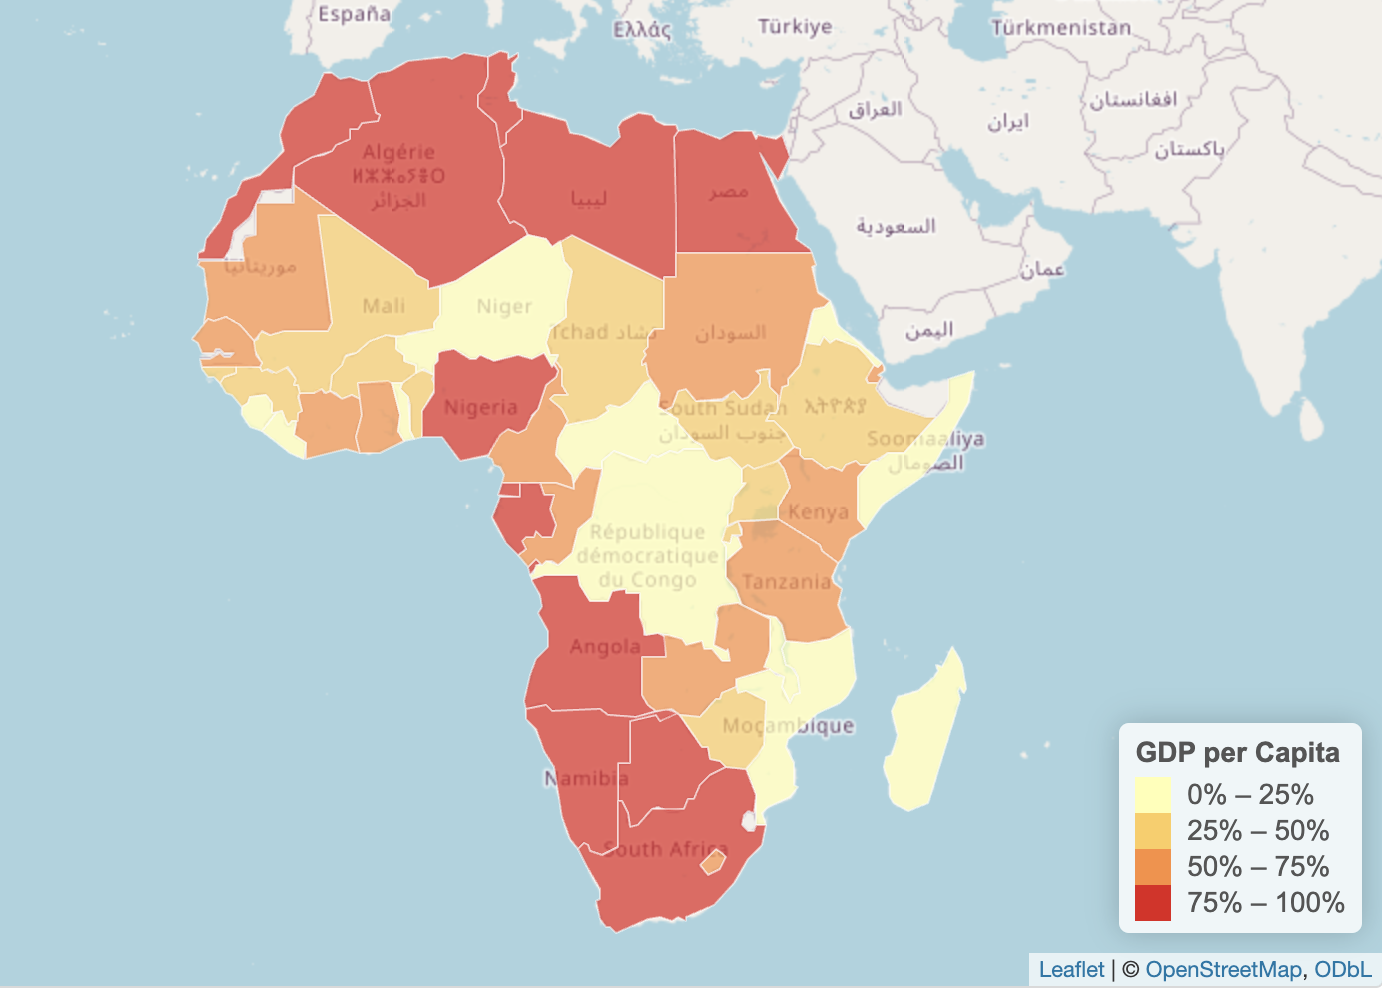
\includegraphics[width=0.7\linewidth]{graphs/map} \end{center}

According to the World Bank's definition, middle-income countries had a
per capita gross national income of more than US\$995.00 in the years
2015--17 {[}ADD CITATION{]}. Among the 35 countries included in our
dataset, 20 are classified as low-income countries, and 15 are
classified as middle-income countries. Additionally, 11 are classified
as countries in Fragile and Conflict-Affected Situations, which, by
definition, have experienced a peacekeeping or peace-building mission
within the last three years.

Sub-Saharan African countries not only differ in terms of economic
prosperity but also in economic structure and resource intensity.
Resource-intensive countries include both oil-exporting nations, where
net oil exports make up 30 percent or more of total exports, and
commodity exporters, where nonrenewable natural resources represent 25
percent or more of total exports. The divergence between
resource-intensive and non-resource-intensive countries became more
entrenched following the commodity price shock of 2015 {[}ADD
CITATION{]}. Non-resource-intensive countries have proven more
resilient, supported by their more diversified economies. On the other
hand, resource-intensive economies generally have a less diversified
structure, making them more susceptible to external shocks. In our
dataset, 6 of the countries are oil exporters, and 11 export other
commodities such as iron ore, copper, cotton, coffee, and sugar. The
remaining 18 countries are non-resource-intensive and their economies
are not reliant on exports.

In recent years, the Sub-Saharan Africa region has grappled with
significant economic challenges, including soaring inflation, pronounced
exchange rate pressures, debt vulnerabilities, and widening economic
disparities within the region. Therefore, addressing these structural
and economic disparities is imperative for tackling developmental issues
in the region.

\hypertarget{data}{%
\section{Data}\label{data}}

In order to continue assessing and enhancing the fairness of the machine
learning models, we use the same Global Findex Database as our
colleagues before us\citep{Porta2022}. The Global Findex database was
first launched in 2011 by the World Bank---with funding from the Bill \&
Melinda Gates Foundation. It is the world's most comprehensive data set
on how adults save, borrow, make payments, and manage risk. The dataset
contains over 200 indicators including account ownership, payments,
savings, credit, and financial resilience and has coverage over 140
nations, representing 97\% of the world's population for year 2017,
2014, and 2011\citep{Demirguc-Kunt2022}.

The data was constructed through a series of surveys carried out by
Gallup, Inc in association with the annual Gallup World Poll. They
randomly sampled 1000 individuals from each country and asked them to
respond to a survey either over the phone or in-person. The target
population is the civilian, non-institutionalized population 15 years
and above. In consistency with the former colleagues, our sample covers
only the Sub-Saharan region (35 countries total), thus there are 35,000
total observations and 105 total variables. Since the sampling was
random and the sample size is large, we can assume that our sample is
representative of the total population of people living in the 35
Sub-Saharan countries in the data. The data was collected directly from
individuals over the 2017 calendar year and is self-contained, meaning
it does not rely on any external resources.

After basic data cleaning, we created a basic summary statistics table
with the mean and standard deviations of each variable.

\begin{longtable}[]{@{}
  >{\raggedright\arraybackslash}p{(\columnwidth - 12\tabcolsep) * \real{0.2366}}
  >{\raggedleft\arraybackslash}p{(\columnwidth - 12\tabcolsep) * \real{0.1183}}
  >{\raggedleft\arraybackslash}p{(\columnwidth - 12\tabcolsep) * \real{0.1075}}
  >{\raggedleft\arraybackslash}p{(\columnwidth - 12\tabcolsep) * \real{0.1505}}
  >{\raggedleft\arraybackslash}p{(\columnwidth - 12\tabcolsep) * \real{0.1398}}
  >{\raggedleft\arraybackslash}p{(\columnwidth - 12\tabcolsep) * \real{0.1290}}
  >{\raggedleft\arraybackslash}p{(\columnwidth - 12\tabcolsep) * \real{0.1183}}@{}}
\caption{Summary Statistics}\tabularnewline
\toprule\noalign{}
\begin{minipage}[b]{\linewidth}\raggedright
X
\end{minipage} & \begin{minipage}[b]{\linewidth}\raggedleft
All..Mean.
\end{minipage} & \begin{minipage}[b]{\linewidth}\raggedleft
All..Std.
\end{minipage} & \begin{minipage}[b]{\linewidth}\raggedleft
Female..Mean.
\end{minipage} & \begin{minipage}[b]{\linewidth}\raggedleft
Female..Std.
\end{minipage} & \begin{minipage}[b]{\linewidth}\raggedleft
Male..Mean.
\end{minipage} & \begin{minipage}[b]{\linewidth}\raggedleft
Male..Std.
\end{minipage} \\
\midrule\noalign{}
\endfirsthead
\toprule\noalign{}
\begin{minipage}[b]{\linewidth}\raggedright
X
\end{minipage} & \begin{minipage}[b]{\linewidth}\raggedleft
All..Mean.
\end{minipage} & \begin{minipage}[b]{\linewidth}\raggedleft
All..Std.
\end{minipage} & \begin{minipage}[b]{\linewidth}\raggedleft
Female..Mean.
\end{minipage} & \begin{minipage}[b]{\linewidth}\raggedleft
Female..Std.
\end{minipage} & \begin{minipage}[b]{\linewidth}\raggedleft
Male..Mean.
\end{minipage} & \begin{minipage}[b]{\linewidth}\raggedleft
Male..Std.
\end{minipage} \\
\midrule\noalign{}
\endhead
\bottomrule\noalign{}
\endlastfoot
gender & 0.5093601 & 0.4999229 & 1.0000000 & 0.0000000 & 0.0000000 &
0.0000000 \\
emp\_in & 0.7003492 & 0.4581147 & 0.6379253 & 0.4806201 & 0.7651548 &
0.4239202 \\
fin2 & 0.1930083 & 0.3946678 & 0.1679055 & 0.3737978 & 0.2190689 &
0.4136331 \\
fin7 & 0.0462749 & 0.2100842 & 0.0388999 & 0.1933644 & 0.0539312 &
0.2258916 \\
fin15 & 0.2158512 & 0.4114202 & 0.1892137 & 0.3916945 & 0.2435051 &
0.4292158 \\
fin16 & 0.1182113 & 0.3228649 & 0.1001817 & 0.3002545 & 0.1369287 &
0.3437869 \\
fin19 & 0.0608304 & 0.2390240 & 0.0498018 & 0.2175442 & 0.0722799 &
0.2589618 \\
fin20 & 0.1725211 & 0.3778407 & 0.1676577 & 0.3735775 & 0.1775701 &
0.3821668 \\
fin21 & 0.1181271 & 0.3227654 & 0.1053023 & 0.3069552 & 0.1314413 &
0.3378969 \\
has\_access & 0.4391065 & 0.4962886 & 0.3703337 & 0.4829140 & 0.5105033
& 0.4999111 \\
fin26 & 0.3301502 & 0.4702769 & 0.2827882 & 0.4503730 & 0.3793192 &
0.4852384 \\
fin28 & 0.3703252 & 0.4829019 & 0.3605880 & 0.4801910 & 0.3804339 &
0.4855143 \\
fin30 & 0.3013336 & 0.4588469 & 0.2895606 & 0.4535772 & 0.3135557 &
0.4639579 \\
fin32 & 0.2550587 & 0.4359034 & 0.2003634 & 0.4002888 & 0.3118409 &
0.4632651 \\
fin37 & 0.0833368 & 0.2763965 & 0.0860588 & 0.2804624 & 0.0805110 &
0.2720944 \\
fin38 & 0.0456439 & 0.2087159 & 0.0447638 & 0.2067934 & 0.0465575 &
0.2106981 \\
fin42 & 0.2566993 & 0.4368213 & 0.2268748 & 0.4188283 & 0.2876618 &
0.4526920 \\
fin48 & 0.7194481 & 0.4492784 & 0.6855798 & 0.4643037 & 0.7546086 &
0.4303375 \\
mobileowner & 0.7032098 & 0.4568529 & 0.6539478 & 0.4757297 & 0.7543514
& 0.4304896 \\
educ\_1 & 0.5268184 & 0.4992908 & 0.5756525 & 0.4942640 & 0.4761211 &
0.4994509 \\
educ\_2 & 0.4348997 & 0.4957543 & 0.3963495 & 0.4891588 & 0.4749207 &
0.4993920 \\
educ\_3 & 0.0382819 & 0.1918801 & 0.0279980 & 0.1649739 & 0.0489582 &
0.2157900 \\
inc\_q\_1 & 0.1594800 & 0.3661308 & 0.1829369 & 0.3866308 & 0.1351282 &
0.3418751 \\
inc\_q\_2 & 0.1721425 & 0.3775122 & 0.1906178 & 0.3928045 & 0.1529624 &
0.3599666 \\
inc\_q\_3 & 0.1864036 & 0.3894402 & 0.1954080 & 0.3965308 & 0.1770556 &
0.3817322 \\
inc\_q\_4 & 0.2109714 & 0.4080067 & 0.2061447 & 0.4045523 & 0.2159822 &
0.4115196 \\
inc\_q\_5 & 0.2710025 & 0.4444867 & 0.2248926 & 0.4175288 & 0.3188716 &
0.4660592 \\
economy\_Benin & 0.0377771 & 0.1906608 & 0.0331186 & 0.1789536 &
0.0426134 & 0.2019925 \\
economy\_Botswana & 0.0376930 & 0.1904567 & 0.0512884 & 0.2205945 &
0.0235788 & 0.1517394 \\
economy\_Burkina Faso & 0.0354634 & 0.1849518 & 0.0222993 & 0.1476613 &
0.0491297 & 0.2161481 \\
economy\_Cameroon & 0.0384923 & 0.1923855 & 0.0398910 & 0.1957111 &
0.0370402 & 0.1888685 \\
economy\_Chad & 0.0360103 & 0.1863196 & 0.0241163 & 0.1534165 &
0.0483581 & 0.2145309 \\
economy\_Congo, Rep. & 0.0342013 & 0.1817498 & 0.0322927 & 0.1767837 &
0.0361828 & 0.1867528 \\
economy\_Cote d'Ivoire & 0.0381557 & 0.1915761 & 0.0231252 & 0.1503073 &
0.0537598 & 0.2255527 \\
economy\_Ethiopia & 0.0363889 & 0.1872597 & 0.0417906 & 0.2001185 &
0.0307811 & 0.1727315 \\
economy\_Gabon & 0.0358420 & 0.1859000 & 0.0327056 & 0.1778724 &
0.0390980 & 0.1938365 \\
economy\_Guinea & 0.0320559 & 0.1761522 & 0.0295672 & 0.1693971 &
0.0346395 & 0.1828727 \\
economy\_Kenya & 0.0411426 & 0.1986241 & 0.0422861 & 0.2012494 &
0.0399554 & 0.1958629 \\
economy\_Lesotho & 0.0371040 & 0.1890207 & 0.0422035 & 0.2010614 &
0.0318100 & 0.1755015 \\
economy\_Madagascar & 0.0411426 & 0.1986241 & 0.0488933 & 0.2156538 &
0.0330961 & 0.1788952 \\
economy\_Malawi & 0.0389550 & 0.1934919 & 0.0510406 & 0.2200897 &
0.0264083 & 0.1603531 \\
economy\_Mali & 0.0370199 & 0.1888145 & 0.0336967 & 0.1804548 &
0.0404699 & 0.1970669 \\
economy\_Mauritania & 0.0299945 & 0.1705757 & 0.0227948 & 0.1492551 &
0.0374689 & 0.1899160 \\
economy\_Mozambique & 0.0369778 & 0.1887113 & 0.0336967 & 0.1804548 &
0.0403841 & 0.1968669 \\
economy\_Namibia & 0.0403853 & 0.1968654 & 0.0531880 & 0.2244174 &
0.0270942 & 0.1623650 \\
economy\_Niger & 0.0362206 & 0.1868426 & 0.0306409 & 0.1723499 &
0.0420132 & 0.2006279 \\
economy\_Rwanda & 0.0396702 & 0.1951873 & 0.0464156 & 0.2103921 &
0.0326674 & 0.1777722 \\
economy\_Senegal & 0.0355475 & 0.1851630 & 0.0329534 & 0.1785221 &
0.0382406 & 0.1917848 \\
economy\_South Africa & 0.0384923 & 0.1923855 & 0.0364222 & 0.1873460 &
0.0406413 & 0.1974664 \\
economy\_South Sudan & 0.0321821 & 0.1764871 & 0.0325405 & 0.1774378 &
0.0318100 & 0.1755015 \\
economy\_Togo & 0.0355896 & 0.1852685 & 0.0275025 & 0.1635491 &
0.0439853 & 0.2050711 \\
economy\_Uganda & 0.0382819 & 0.1918801 & 0.0424513 & 0.2016247 &
0.0339535 & 0.1811174 \\
economy\_Zambia & 0.0391654 & 0.1939923 & 0.0449290 & 0.2071567 &
0.0331819 & 0.1791189 \\
economy\_Zimbabwe & 0.0400488 & 0.1960778 & 0.0481500 & 0.2140919 &
0.0316385 & 0.1750433 \\
\end{longtable}

We also created various visualizations to help understand who is in the
data and acknowledge potential sources of bias within the data.

\hypertarget{outcome-variable-of-interest-access-to-emergency-fund-fin24}{%
\subsection{\texorpdfstring{\emph{Outcome Variable of Interest: Access
to Emergency Fund
(Fin24)}}{Outcome Variable of Interest: Access to Emergency Fund (Fin24)}}\label{outcome-variable-of-interest-access-to-emergency-fund-fin24}}

The variable ``Fin24'' in the dataset asked participants the question:
Now, imagine that you have an emergency and you need to pay {[}1/20 of
GNI per capita in local currency{]}. Is it possible or not possible that
you could come up with {[}1/20 of GNI per capita in local currency{]}
within the NEXT MONTH\citep{Demirguc-Kunt2022}? In order to make it more
straightforward for interpretations, we restrict the response into a
binary variable for Yes and No.~The overall distribution of access to
emergency funds showed 17,599 individuals had access to emergency funds
while 14,342 did not. This indicates that over half of individuals
represented in the data do not have access to emergency funds.

To help conceptually understand how the outcome variables might vary
among different levels of the variables, we chose 50 \% as the benchmark
proportion for checking if the possibility of coming up with emergency
funds for each variable group of interest is different from a random
50/50 chance.

\begin{figure}

{\centering 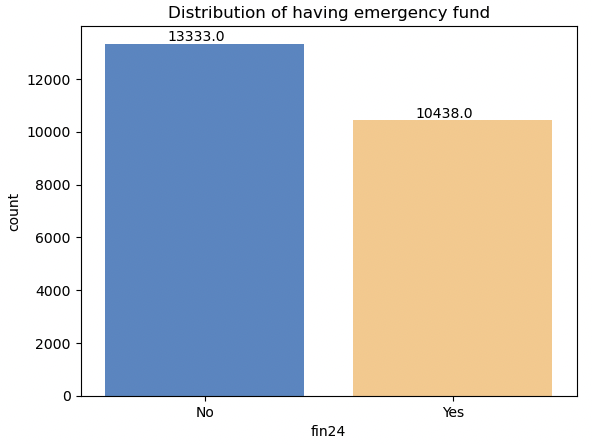
\includegraphics[width=0.7\linewidth]{graphs/f24_graph1} 

}

\caption{Distribution of having emergency fund}\label{fig:unnamed-chunk-4}
\end{figure}

\hypertarget{demographics}{%
\subsection{Demographics}\label{demographics}}

\hypertarget{protected-attribute-of-focus-gender-female}{%
\subsubsection{\texorpdfstring{\emph{Protected Attribute of Focus:
Gender
(female)}}{Protected Attribute of Focus: Gender (female)}}\label{protected-attribute-of-focus-gender-female}}

The variable ``female'' distinguishes gender. There are 12,108 females
and 11,663 males in the dataset. It appears to have a fair distribution
between different genders for the dataset as a whole.

\begin{figure}

{\centering 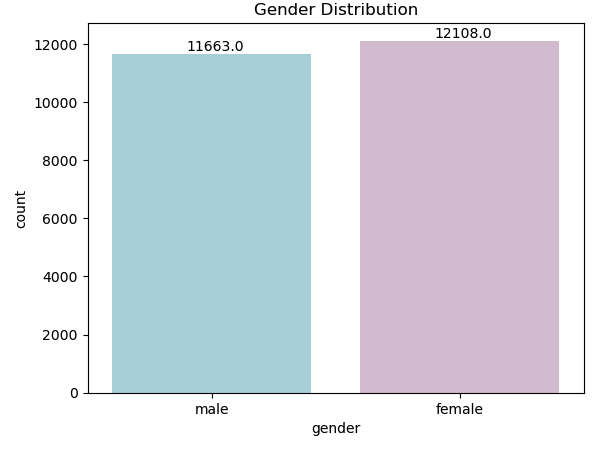
\includegraphics[width=1\linewidth]{graphs/f24_graph2} 

}

\caption{Distribution on gender}\label{fig:unnamed-chunk-5}
\end{figure}

While it looks quite balanced in the previous figure, we observe a
discrepancy between the two genders when compared against our outcome
variable of interest. Females have a 15\% lower chance of having access
to emergency funds.

\begin{figure}

{\centering 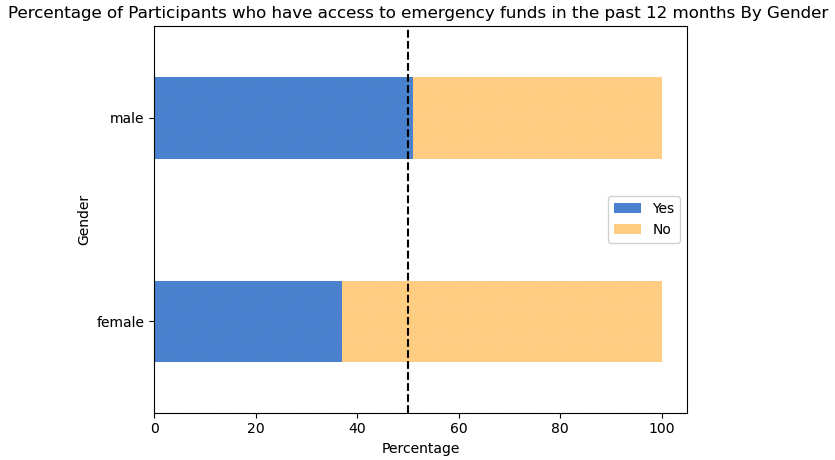
\includegraphics[width=1\linewidth]{graphs/f24_graph3} 

}

\caption{Distribution of having emergency fund by gender}\label{fig:unnamed-chunk-6}
\end{figure}

In order to investigate further into how discrepancy of gender plays
into other predictor variables, we created visuals for contrasting the
two genders.

\hypertarget{education-educ}{%
\subsubsection{\texorpdfstring{\emph{Education
(educ)}}{Education (educ)}}\label{education-educ}}

The variable ``educ'' distinguishes education level among participants:
1 being the completed primary education or less, 2 being completed
secondary education, and 3 being completed tertiary education. The
majority in the dataset is participants with primary or less education
(12523 participants). On the other hand, there are only 910 participants
who have tertiary education. Overall, the discrepancy between education
levels appears quite drastic, and might result in a varying prediction
for access to emergency funds. If we break down education by gender, we
see that more females than males have primary or less education while
the opposite for secondary or tertiary education.

\begin{figure}

{\centering 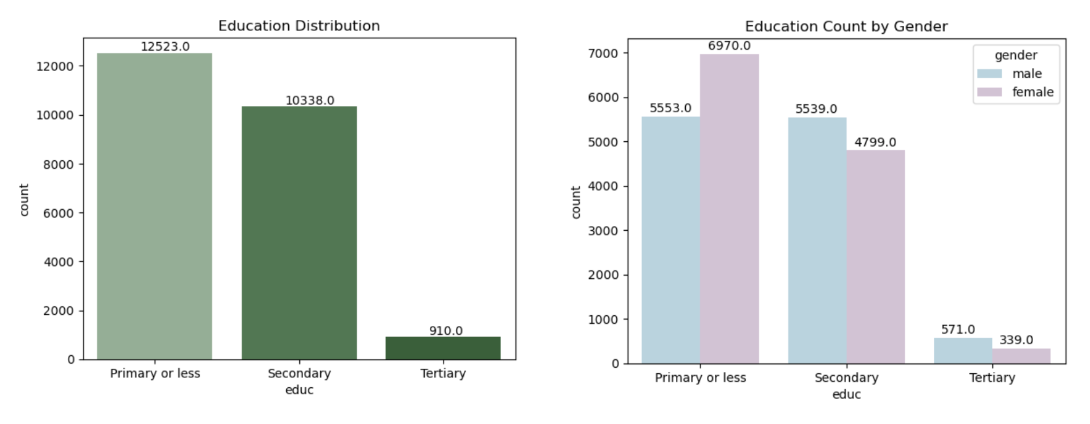
\includegraphics[width=1\linewidth]{graphs/f24_graph4} 

}

\caption{Distribution by education level}\label{fig:unnamed-chunk-7}
\end{figure}

When we consider gender and education with respect to the outcome
variable of interest, we observe that tertiary education levels have the
highest likelihood of access to emergency funds while primary education
is the least likely.

\begin{figure}

{\centering 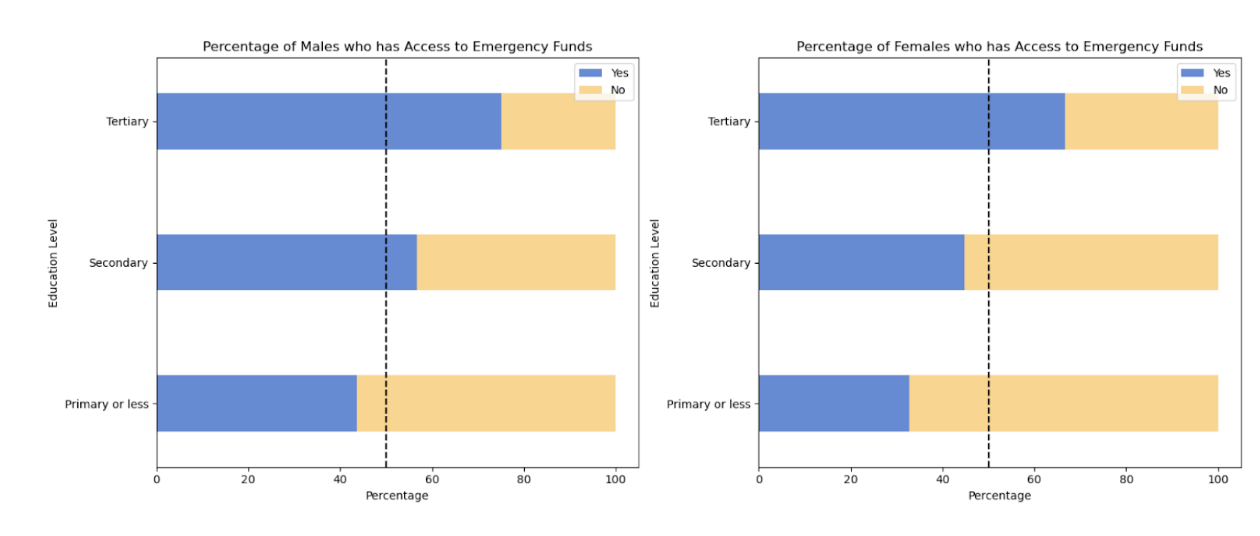
\includegraphics[width=1\linewidth]{graphs/f24_graph5} 

}

\caption{Distribution of access to emergency funds by education level and gender}\label{fig:unnamed-chunk-8}
\end{figure}

This discrepancy between education levels is reasonable since
participants with tertiary education might have been more financially
independent and have higher financial resilience, thus be more likely to
have access to emergency funds. Nonetheless, we continue to observe that
females have a lower access to emergency funds, among the same education
level. It shows that gender imbalance is still evident when we position
it in relationship to other predictors.

\hypertarget{income-quantile-inc_q}{%
\subsubsection{\texorpdfstring{\emph{Income Quantile
(Inc\_q)}}{Income Quantile (Inc\_q)}}\label{income-quantile-inc_q}}

The variable ``inc\_q'' distinguishes the income quintile within an
economy. It is separated into 5 quantiles with 1 being the poorest and 5
being the richest. Income quintile 5, or the richest 20\%, is the
largest quantile. There are more male than females in the richest 20\%
quintile, while females compose the majority of the poorest 20\%, second
poorest 20\%, and middle 20\%, which are the poorest quantiles.

\begin{figure}

{\centering 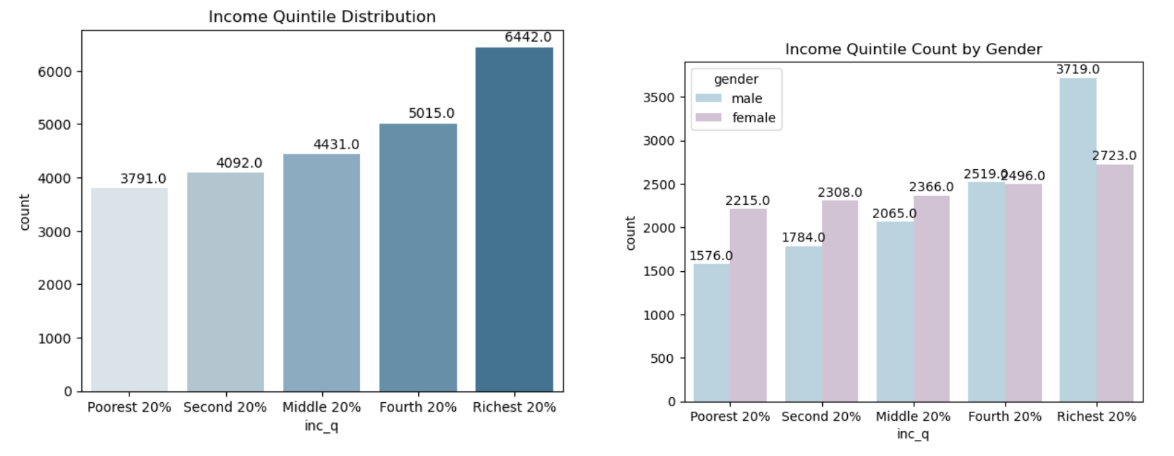
\includegraphics[width=1\linewidth]{graphs/income_graph6} 

}

\caption{Income Quantile Distribution}\label{fig:unnamed-chunk-9}
\end{figure}

We observe a similar gradient in access to emergency funds among the
different income quintiles. This discrepancy is expected since
participants with the level of income are directly related to financial
stability and resilience. However, the gap between females and male is
still concerning: male that are in the top two income quintile will have
at least 50\% chance of access to emergency funds, whereas only females
that are the top 1 income quintile will have a comparable likelihood.

\begin{figure}

{\centering 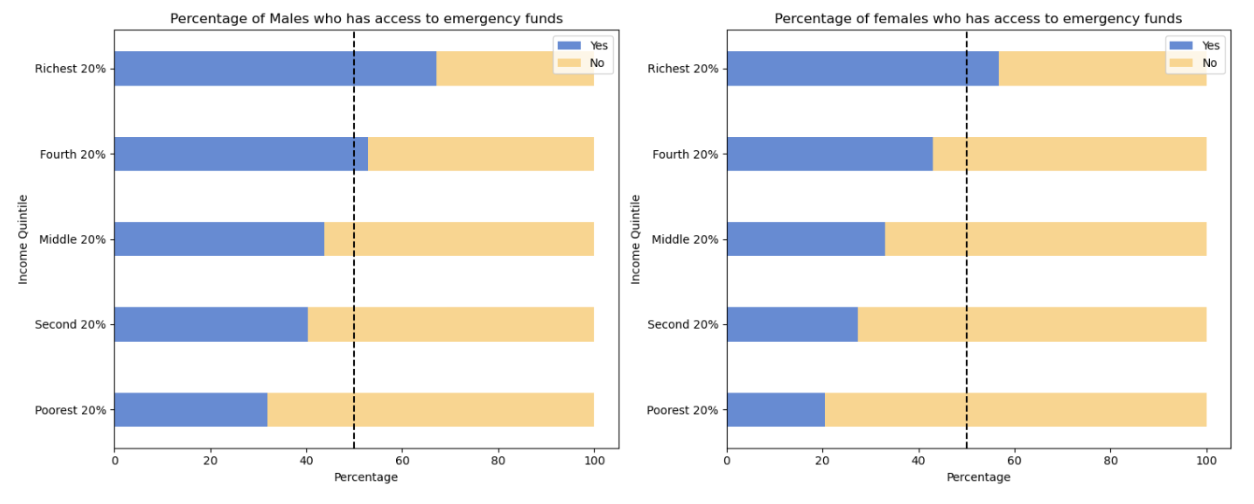
\includegraphics[width=1\linewidth]{graphs/employ_graph7} 

}

\caption{Distribution of access to emergency funds by income quantiile and gender}\label{fig:unnamed-chunk-10}
\end{figure}

\hypertarget{employment-status-emp_in}{%
\subsubsection{\texorpdfstring{\emph{Employment Status
(emp\_in)}}{Employment Status (emp\_in)}}\label{employment-status-emp_in}}

Employment Status asks whether or not the participant is in the
workforce. There are 16648 individuals who were in the workforce while
7123 were not, and more females are out of the workforce than males,
thus suggesting that females are less likely to achieve economic
independence than males.

\begin{figure}

{\centering 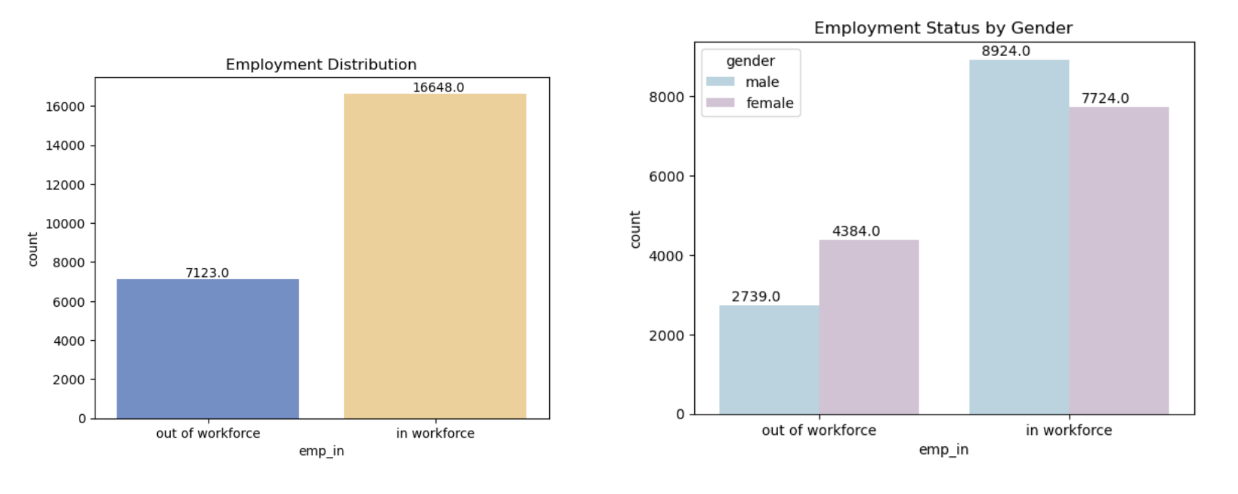
\includegraphics[width=1\linewidth]{graphs/employ_graph8} 

}

\caption{Distribution of employment status}\label{fig:unnamed-chunk-11}
\end{figure}

The disparity between females and male is quite alarming when we break
it down by employment status. Regardless of the employment status,
females do not even have a 50\% chance of having access to emergency
funds.

\begin{figure}

{\centering 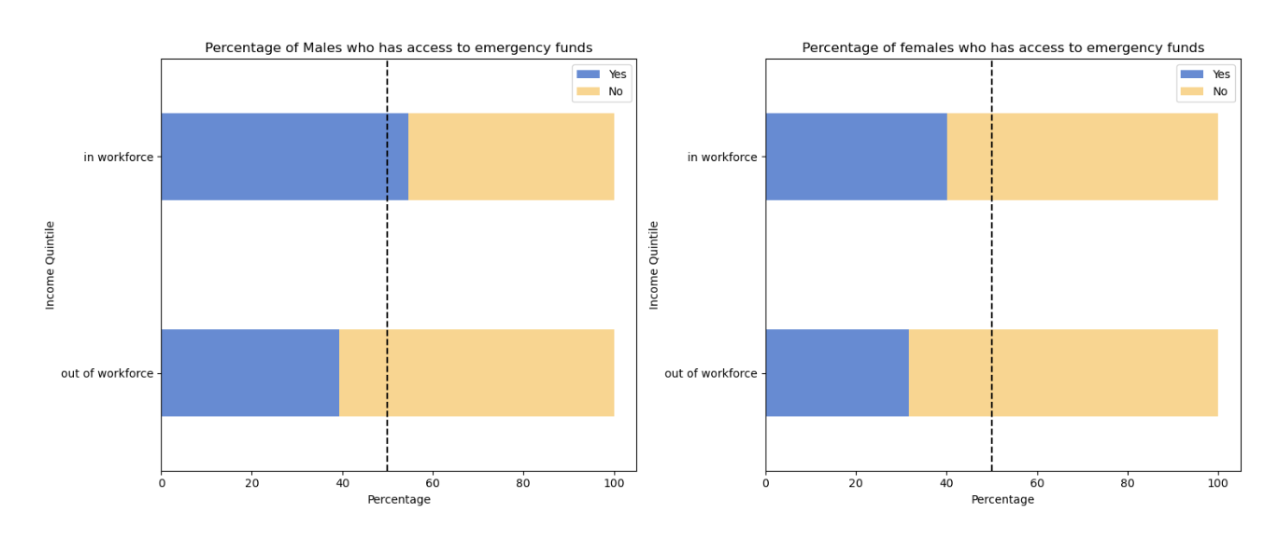
\includegraphics[width=1\linewidth]{graphs/employ_graph9} 

}

\caption{Distribution of access to emergency funds by employment status and gender}\label{fig:unnamed-chunk-12}
\end{figure}

\hypertarget{country-economy}{%
\subsubsection{\texorpdfstring{\emph{Country
(economy)}}{Country (economy)}}\label{country-economy}}

The ``economy'' variable represents the country that the participants
live in. There are 27 different countries from Sub-Saharan Africa with
around 800-900 respondents each. The countries included are Benin,
Botswana, Burkina Faso, Cameroon, Central African Republic, Chad, Congo
Dem. Rep.~Congo Rep., Côte d'Ivoire, Ethiopia, Gabon, Ghana, Guinea,
Kenya, Lesotho, Liberia, Madagascar, Malawi, Mali, Mauritania,
Mozambique, Namibia, Niger, Nigeria, Rwanda, Senegal, Sierra Leone,
South Africa, South Sudan, Tanzania, Togo, Uganda, Zambia, and Zimbabwe.

While looking at the outcome variable of interest broken down by country
and gender, we see that Liberia has the highest proportion of both
females and male having access to emergency funds, while Zambia has the
lowest proportion of accessing emergency funds in both females and
males. It's also important to note that the difference between males and
females is largest in countries like Botswana and Kenya.

\begin{figure}

{\centering 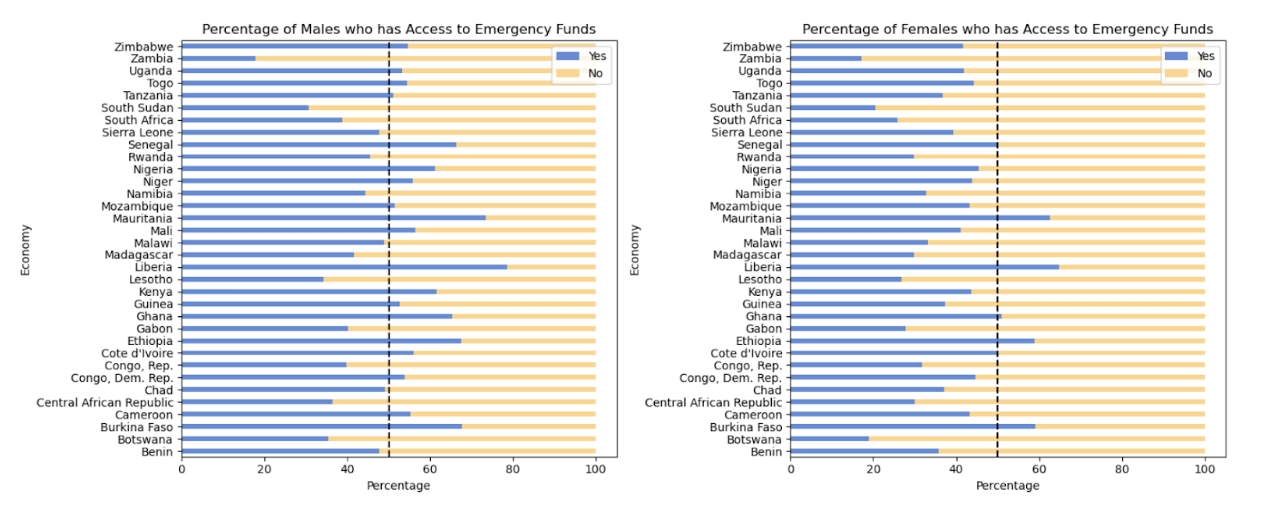
\includegraphics[width=1\linewidth]{graphs/country_graph10} 

}

\caption{Distributions of Access to Emergency Funds by country and gender}\label{fig:unnamed-chunk-13}
\end{figure}

We iterate the visualizations for each main financial variable of
interest in the dataset by gender, by gender and economy, and by gender
and education level, to check if there's recurring discrepancy among
genders. Due to the page constraints, we decide to not include all
visualizations and attach our Jupyter Notebook
(\href{https://drive.google.com/file/d/1f9AauOn4I2Rl5io_viMw0WbEXKFiJcRA/view?usp=sharing}{link})
for reference.

\hypertarget{financial-variables}{%
\subsection{Financial Variables}\label{financial-variables}}

We describe financial variables that are likely to have an impact on
access to emergency fund in the following section.

\hypertarget{has-a-debit-card-fin2}{%
\subsubsection{\texorpdfstring{\emph{Has a debit card
(fin2)}}{Has a debit card (fin2)}}\label{has-a-debit-card-fin2}}

The variable ``fin2'' inquired whether participants possessed ``a card
connected to an account at a financial institution that allows immediate
withdrawals of money.'' We posit that this variable correlates with the
outcome, as a debit card serves both saving and withdrawal purposes,
closely intertwining with income accumulation. The absence of a debit
card signifies a lack of savings and financial stability, potentially
hindering the ability to build emergency funds. Among all participants,
4,588 individuals own a debit card, while 19,183 individuals do not,
surpassing the number of cardholders by more than five times. Despite
this significant difference, the distribution by gender indicates a
relatively similar percentage of males and females owning a debit card.
This suggests no conspicuous imbalance in debit card ownership between
genders.

\hypertarget{has-a-credit-card-fin7}{%
\subsubsection{\texorpdfstring{\emph{Has a credit card
(fin7)}}{Has a credit card (fin7)}}\label{has-a-credit-card-fin7}}

The variable ``fin7'' asked whether participants possessed ``a card that
allows borrowing to make payments and pay the balance off later.'' We
hypothesize that this variable correlates with the outcome, as a credit
card facilitates immediate access to funds during emergencies and
provides flexible repayment options. Notably, only 1,100 individuals,
comprising less than 5\% of all participants, own a credit card. Despite
this contrast, the distribution by gender reveals a relatively similar
percentage of males and females owning a credit card. This implies no
apparent gender-based imbalance in credit card ownership.

\hypertarget{saved-for-farmbusiness-purposes-in-the-past-12-months-fin15}{%
\subsubsection{\texorpdfstring{\emph{Saved for farm/business purposes in
the past 12 months
(fin15)}}{Saved for farm/business purposes in the past 12 months (fin15)}}\label{saved-for-farmbusiness-purposes-in-the-past-12-months-fin15}}

The variable ``fin15'' asks whether respondents saved money to ``start,
operate, or grow a business or farm in the past 12 months.'' We propose
that this variable may correlate with the outcome, as saving for
business or farm endeavors suggests a proactive approach towards
entrepreneurship or agricultural ventures. Among all participants, 5,131
individuals saved money for business or farm purposes, while 18,640
individuals did not. Examining the gender composition, there is a
slightly larger percentage of males who engaged in saving for business
or farm compared to females. This observation suggests a gender
difference in the inclination to save for entrepreneurial or
agricultural pursuits within the surveyed population (5\%).

\hypertarget{saved-for-old-age-in-the-past-12-months-fin16}{%
\subsubsection{\texorpdfstring{\emph{Saved for old age in the past 12
months
(fin16)}}{Saved for old age in the past 12 months (fin16)}}\label{saved-for-old-age-in-the-past-12-months-fin16}}

The variable ``fin16'' inquires whether respondents saved money for old
age in the past 12 months. We propose that this variable may correlate
with the outcome, as saving for old age reflects a forward-thinking
approach to financial planning and retirement readiness. Among all
participants, only 2,810 individuals, constituting a distinct subset,
saved money for old age, while 20,961 individuals did not. Analyzing the
gender composition, there is a slightly larger percentage of males who
engaged in saving for old age compared to females (3.6\%). This
observation resonates with the trend identified in the variable fin15.
These findings collectively suggest a gender difference in the
propensity to save for specific financial goals within the surveyed
population.

\hypertarget{has-loan-from-a-financial-institution-for-home-apartment-or-land-fin19}{%
\subsubsection{\texorpdfstring{\emph{Has loan from a financial
institution for home, apartment, or land
(fin19)}}{Has loan from a financial institution for home, apartment, or land (fin19)}}\label{has-loan-from-a-financial-institution-for-home-apartment-or-land-fin19}}

The variable `fin19' signifies whether a respondent by themself or with
someone else currently has a loan that they took out from a bank or
another type of formal financial institution to purchase a home,
apartment or land. We suspect that the ability to access emergency funds
would be impeded by having a loan, because a part of the income would
have to be channeled towards repayment. On the other hand, an unspent
loan amount could become an emergency fund. In our random sample, 22,325
respondents did not have a loan from a financial institution for a home,
apartment, or land, whereas only 1,446 respondents did. In terms of the
gender composition, of the respondents who had a loan, there is a
slightly larger percentage of males by 2.3\% compared to females.

\hypertarget{borrowed-in-past-12-months-for-medical-purposes-fin20}{%
\subsubsection{\texorpdfstring{\emph{Borrowed in past 12 months: for
medical purposes
(fin20)}}{Borrowed in past 12 months: for medical purposes (fin20)}}\label{borrowed-in-past-12-months-for-medical-purposes-fin20}}

The variable `fin20' signifies whether a respondent by themself or
together with someone else has borrowed money for health or medical
purposes in the last 12 months. We suspect that the ability to access
emergency funds would be impeded by having borrowed, because a part of
the income would have to be channeled towards repayment. Moreover, since
the respondent is borrowing for medical purposes, their productivity to
generate emergency funds could be argued due to potential illness. In
our random sample, 19,670 respondents had not borrowed for medical
purposes, whereas only 4,101 respondents did. In terms of the gender
composition in the respondents who had borrowed, there is a slightly
larger percentage of males by 1\% compared to females.

\hypertarget{borrowed-for-farmbusiness-purposes-in-past-12-months-fin21}{%
\subsubsection{\texorpdfstring{\emph{Borrowed for farm/business purposes
in past 12 months
(Fin21)}}{Borrowed for farm/business purposes in past 12 months (Fin21)}}\label{borrowed-for-farmbusiness-purposes-in-past-12-months-fin21}}

The variable `fin21' signifies whether a respondent by themself or
together with someone else has borrowed money to start, operate, or grow
a business or farm in the last 12 months. Similar to our argument for
Fin20, we suspect that the ability to access emergency funds would be
impeded by having borrowed, because a part of the income would have to
be channeled towards repayment. In our random sample, 20,963 respondents
had not borrowed for medical purposes, whereas only 2,808 respondents
did. In terms of the gender composition in the respondents who had
borrowed, there is a slightly larger percentage of males by 2.9\%
compared to females.

\hypertarget{sent-domestic-remittances-in-past-12-months-fin26}{%
\subsubsection{\texorpdfstring{\emph{Sent domestic remittances in past
12 months
(Fin26)}}{Sent domestic remittances in past 12 months (Fin26)}}\label{sent-domestic-remittances-in-past-12-months-fin26}}

The variable `fin26' signifies whether a respondent has personally given
or sent money to a relative or friend living in a different city or area
inside the country in the past 12 months. The money can be given or sent
for any reason, and can be money that the respondent brought or sent in
some other way. We suspect that the ability to access emergency funds
would be encouraged by having voluntarily sent domestic remittances. We
hypothesize that the sender of remittances would be less able to access
emergency funds given the outflow of their money. In our random sample,
15,923 respondents had not borrowed for medical purposes, whereas only
7,848 respondents did. In terms of the gender composition in the
respondents who had sent domestic remittances, there is a larger
percentage of males by approximately 9\% compared to females.

\hypertarget{received-domestic-remittance-in-the-past-12-months-fin28}{%
\subsubsection{\texorpdfstring{\emph{Received Domestic Remittance in the
past 12 months
(fin28)}}{Received Domestic Remittance in the past 12 months (fin28)}}\label{received-domestic-remittance-in-the-past-12-months-fin28}}

The variable `fin28' asks whether the respondent has received money from
a relative or friend living in a different city or area within the
country where the survey is conducted, excluding payments for goods and
services, in the past 12 months, requiring a ``Yes'' or ``No'' response.
We believe that this variable is correlated with the outcome variable
because this variable provides insight into the respondent's potential
support network and access to financial resources that could be utilized
in case of an emergency. In our random sample, 8,803 respondents
received domestic remittance in the past 12 months while 14698
respondents did not. In the graph, slightly more male respondents
received domestic remittances compared to females (\textasciitilde2\%).

\hypertarget{received-government-transfer-in-the-past-12-months-fin37}{%
\subsubsection{\texorpdfstring{\emph{Received Government Transfer in the
past 12 months
(fin37)}}{Received Government Transfer in the past 12 months (fin37)}}\label{received-government-transfer-in-the-past-12-months-fin37}}

The variable ``fin37'' asks respondents whether they have personally
received any financial support from the government in the past 12
months, including payments for educational or medical expenses,
unemployment benefits, subsidy payments, or any type of social benefits,
excluding wages or work-related payments. This information is crucial as
individuals who have received government financial support may have a
higher likelihood of being able to access emergency funds, as they may
have access to additional resources or assistance programs. In our
random sample, only 1,981 respondents received government transfer,
while 21,790 respondents did not. There's no observable difference
between male and female respondents (\textasciitilde0.5\%).

\hypertarget{received-government-pension-in-the-past-12-months-fin38}{%
\subsubsection{\texorpdfstring{\emph{Received Government Pension in the
past 12 months
(fin38)}}{Received Government Pension in the past 12 months (fin38)}}\label{received-government-pension-in-the-past-12-months-fin38}}

The variable `fin38' asks respondents whether they have personally
received a pension from the government, military, or public sector in
the past 12 months. It is highly related to the outcome variable as
individuals receiving pensions may have a stable source of income that
could contribute to their ability to access emergency funds. Therefore,
the presence or absence of pension income may influence respondents'
perceptions of their financial security and ability to meet emergency
financial needs. In the random sample, only 1,085 respondents received
government pension, while 22,686 respondents did not. There's no
observable difference between male and female respondents
(\textasciitilde0.2\%).

\hypertarget{having-a-national-id-fin48}{%
\subsubsection{\texorpdfstring{\emph{Having a national ID
(fin48)}}{Having a national ID (fin48)}}\label{having-a-national-id-fin48}}

The variable `fin48' asks respondents whether they own a national id of
the country where the survey is conducted. The possession of a national
ID can significantly impact individuals' access to financial services,
eligibility for government assistance programs, and employment
opportunities. Having a national ID may facilitate the process of
obtaining emergency funds by providing access to formal financial
institutions, qualifying for social benefits, and streamlining identity
verification for transactions, thereby influencing the respondent's
ability to meet emergency financial needs within the next month. In the
random sample, 72\% of respondents owns a national ID of the country
where the survey is conducted. There's an observable 10\% difference
between male and females, where 10\% more males owns a national ID.

\hypertarget{paid-utility-bills-in-past-12-months-fin30}{%
\subsubsection{\texorpdfstring{\emph{Paid utility bills in past 12
months
(fin30)}}{Paid utility bills in past 12 months (fin30)}}\label{paid-utility-bills-in-past-12-months-fin30}}

The variable ``fin30'' asked the participants if they have ``personally,
made regular payments for electricity, water, OR trash collection?'' We
believe this variable is correlated with the outcome since utility bills
are typically recurring expenses that are essential for maintaining
basic needs. If someone struggles to pay their utility bills, it could
indicate that they are living paycheck to paycheck or facing financial
strain. In such situations, they may not have the financial flexibility
to save for emergencies. In our data, only 9,175 individuals paid
utility bills while 22,766 did not. However when we look at the
breakdown by gender, male and female have approximately equal
proportions which suggest that genders may not directly affect the
distribution for the variable.

\hypertarget{received-wage-payment-fin32}{%
\subsubsection{\texorpdfstring{\emph{Received Wage Payment
(fin32)}}{Received Wage Payment (fin32)}}\label{received-wage-payment-fin32}}

The variable ``fin32'' asked the participants if they have
``\ldots received any money from an EMPLOYER, in the form of SALARY OR
WAGES, for doing work in the PAST 12 MONTHS?'' We believe this variable
could be necessary for the model because receiving wage payments is one
important source of saving for emergency funds. Only 6063 individuals
receive wage payments while 17708 do not.There's a visible 10\%
difference between Male receiving wage payments compared to Female.

\hypertarget{own-a-mobile-phone-mobileowner}{%
\subsubsection{\texorpdfstring{\emph{Own a Mobile Phone
(mobileowner)}}{Own a Mobile Phone (mobileowner)}}\label{own-a-mobile-phone-mobileowner}}

The variable ``mobileowner'' is a binary variable where 1 means owns a
mobile phone and 0 otherwise. We believe this variable should be
included for fitting the model because having a mobile phone enables
individuals to quickly reach out for help or access important financial
resources, such as online banking or emergency assistance services to
address unexpected expenses promptly. The majority of the sample owns a
mobile phone, and a slightly higher proportion among male participants.

\hypertarget{received-agricultural-payments-in-past-12-months-fin42}{%
\subsubsection{\texorpdfstring{\emph{Received agricultural payments in
past 12 months
(fin42)}}{Received agricultural payments in past 12 months (fin42)}}\label{received-agricultural-payments-in-past-12-months-fin42}}

The variable ``fin42'' asked the participants if they have
``\ldots received money from any source for the sale of agricultural
products, crops, produce, or livestock in the PAST 12 MONTHS?'' We
believe this variable could be necessary for the model because receiving
agricultural payments is one important source of saving for emergency
funds, especially for resource-intensive countries. In the sample, 6102
individuals receive agricultural payments while 17669 do not. There's a
slightly higher proportion of male receiving agricultural payments than
females.

\hypertarget{summary}{%
\section{Summary}\label{summary}}

Overall, our exploratory data analysis (EDA) reveals that there are
disparities in the outcome variable access to emergency funds, most
significantly with the protected attributes of gender. This choice is
not meant to diminish the importance of the other demographic
disparities that also have an influence on the access to emergency
funds. Nonetheless, the visualizations above show how gender differences
persist in all of these features. Therefore, we believe that choosing
gender as our primary attribute and addressing the gender imbalance
would potentially address the discrepancy we see in the other
attributes. Future research could consider addressing multiple protected
attributes. In terms of other financial variables, through these
visualizations and analysis, we observe that gender differences are less
of a concern than the outcome variable, with around an average of 5\% or
less difference, only with few exceptions like Fin 26 and Fin32 that
have a more visible difference of 10\%. This helps substantiate our
future effort of artificially creating synthetic data that includes more
``Yes'' to female observations while randomly assigning values to other
financial variables.

Having identified the limitations in the data, our next step is to
create a baseline machine learning model and assess the model with
fairness metrics to determine the best model fit. After that, we aim to
improve the model further with synthetic data to further minimize the
bias.

\hypertarget{methods}{%
\section{Methods}\label{methods}}

For our project, we used the programming language Python on Jupyter
Notebook. We collaborated through Google Colab, Google Drive and GitHub.
To clean our data and make preliminary visualizations, we used the
pandas, matplotlib, numpy packages. To explore chi correlation and logit
regression for the statistical component of our EDA, we used
statsmodels.api and chi2\_contingency method from scipy.stats package.
To explore different baseline machine learning models, we mainly used
the sklearn packages to instantiate the models and construct the
confucian matrices.

\hypertarget{exploratory-data-analysis-eda}{%
\subsection{Exploratory Data Analysis
(EDA)}\label{exploratory-data-analysis-eda}}

The EDA helps us understand who is represented in the data and aids in
approaching our final research problem: understanding the factors
contributing to an individual's ability to access and/or generate
emergency funds.

The data set has 105 variables. Hence, the first task at hand was to
narrow down the pool of potential features of interest to our research
problem and analysis. Firstly, we chose our demographic features of
interest that were gender, education level, employment status, income
quintile, and economy. These variables are synonymous to protected or
sensitive attributes. As previously mentioned, an outcome (of an
algorithm) is not considered fair or just, if they are determined mainly
based on a protected attribute. While reading the data description, we
saw that some variables are follow-up questions to the previous
variables. For example, ``fin8'' is only asked if the respondent has an
account at a financial institution OR has a debit card in their name
which is connected to an account. Due to its lack of response completion
in those ``sub-questions'', we filtered out variables where more than
25\% of the entries were NA. We then filtered out those that have
unclear entries labels. For example, the variable ``saved'' and
``borrowed'' have unclear labels for its entry of 1 and 0. Although it
may be reasonable to assume that 1 would indicate yes and 0 otherwise,
we decided to exclude them for the current sprint. Finally, we
shortlisted our potential predictor down to 16 variables. We built on
the previous group's work by exploring countries for each of the 16
financial variables, because we wanted to see to what extent each
variable had predictive power for the outcome variables.

After selecting a pool of features we were interested to explore, we
standardized the data by re-coding it. In the survey, for specially
financial features, respondents either answered `Yes', `No', `Don't
Know' or `Refuse'. We filtered out `Don't Know' and `Refuse' responses
for our variables, because given the low proportion of those responses
for a question, we were skeptical of overfitting and have little
relevance to our research problem. After re-coding, every financial
variable as well as the outcome are now binary, where 1 indicates yes to
the survey questions and 0 indicates no. We want to mention that these
steps are in agreement with the data cleaning methodology implemented by
the previous colleagues.

We visualized the characteristics of the population included in the
data, through multivariate bar-plots. For each of the features we chose,
we created plots displaying the proportion of the respondents who said
``Yes'' or ``No'' for a financial variable, for example, fin2 (Owns a
debit card) for gender, education level and country. We performed this
analysis on all of our shortlisted variables of interest. The main aim
of this approach to our EDA was to investigate any potential
discrepancies between the responses of male and female, primary,
secondary and tertiary education and each country.

After visualization, we decided to enhance our EDA with two statistical
components. First, we ran logit regression with our binary outcome
variable i.e.~access to emergency funds. Our first regression
specification in Fig EDA.1 shows that males have a 4.2 percentage points
higher likelihood of having access to emergency funds than their female
counterparts with statistical significance. This regression suffers from
omitted variable bias (OVB) and we suspect that the impact of gender on
access to emergency funds is underestimated.

\begin{longtable}[]{@{}lrrrrrr@{}}
\caption{Logit 1 Regression Results}\tabularnewline
\toprule\noalign{}
X & coef & std.err & z & P..z. & X.0.025 & X0.975. \\
\midrule\noalign{}
\endfirsthead
\toprule\noalign{}
X & coef & std.err & z & P..z. & X.0.025 & X0.975. \\
\midrule\noalign{}
\endhead
\bottomrule\noalign{}
\endlastfoot
gender\_male & 0.042 & 0.019 & 2.268 & 0.023 & 0.006 & 0.078 \\
\end{longtable}

In our second specification in Fig EDA.2 where we take into account the
economy and education level features (which are the two other protected
attributes that we explored), the likelihood of access to emergency
funds is, on average, 34.75 percentage points higher for men with
primary education from Benin than for comparable females with
statistical significance. In other words, the reference category is an
average male from Benin with primary education These results further
emphasize that gender does have an impact on access to emergency funds
where females are disadvantaged. Furthermore, these results emphasize
that higher levels of education result in greater access of emergency
funds with statistical significance, holding all else constant, which
confirms our initial hypothesis.

\begin{longtable}[]{@{}
  >{\raggedright\arraybackslash}p{(\columnwidth - 12\tabcolsep) * \real{0.3099}}
  >{\raggedleft\arraybackslash}p{(\columnwidth - 12\tabcolsep) * \real{0.1127}}
  >{\raggedleft\arraybackslash}p{(\columnwidth - 12\tabcolsep) * \real{0.1127}}
  >{\raggedleft\arraybackslash}p{(\columnwidth - 12\tabcolsep) * \real{0.1127}}
  >{\raggedleft\arraybackslash}p{(\columnwidth - 12\tabcolsep) * \real{0.0845}}
  >{\raggedleft\arraybackslash}p{(\columnwidth - 12\tabcolsep) * \real{0.1549}}
  >{\raggedleft\arraybackslash}p{(\columnwidth - 12\tabcolsep) * \real{0.1127}}@{}}
\caption{Logit 2 Regression Results}\tabularnewline
\toprule\noalign{}
\begin{minipage}[b]{\linewidth}\raggedright
X
\end{minipage} & \begin{minipage}[b]{\linewidth}\raggedleft
coef
\end{minipage} & \begin{minipage}[b]{\linewidth}\raggedleft
std.err
\end{minipage} & \begin{minipage}[b]{\linewidth}\raggedleft
z
\end{minipage} & \begin{minipage}[b]{\linewidth}\raggedleft
P..z.
\end{minipage} & \begin{minipage}[b]{\linewidth}\raggedleft
X.0.025
\end{minipage} & \begin{minipage}[b]{\linewidth}\raggedleft
X0.975.
\end{minipage} \\
\midrule\noalign{}
\endfirsthead
\toprule\noalign{}
\begin{minipage}[b]{\linewidth}\raggedright
X
\end{minipage} & \begin{minipage}[b]{\linewidth}\raggedleft
coef
\end{minipage} & \begin{minipage}[b]{\linewidth}\raggedleft
std.err
\end{minipage} & \begin{minipage}[b]{\linewidth}\raggedleft
z
\end{minipage} & \begin{minipage}[b]{\linewidth}\raggedleft
P..z.
\end{minipage} & \begin{minipage}[b]{\linewidth}\raggedleft
X.0.025
\end{minipage} & \begin{minipage}[b]{\linewidth}\raggedleft
X0.975.
\end{minipage} \\
\midrule\noalign{}
\endhead
\bottomrule\noalign{}
\endlastfoot
gender\_male & 0.3429 & 0.028 & 12.351 & 0.000 & 0.2890000 & 0.397 \\
educ\_Secondary & 0.6402 & 0.030 & 21.158 & 0.000 & 0.5810000 & 0.700 \\
educ\_Tertiary & 1.8447 & 0.083 & 22.219 & 0.000 & 1.6820000 & 2.007 \\
economy\_Botswana & -1.8396 & 0.084 & -21.824 & 0.000 & -2.0050000 &
-1.674 \\
economy\_Burkina Faso & 0.1494 & 0.077 & 1.950 & 0.051 & -0.0010000 &
0.300 \\
economy\_Cameroon & -0.5553 & 0.070 & -7.885 & 0.000 & -0.6930000 &
-0.417 \\
economy\_Chad & -0.6431 & 0.073 & -8.808 & 0.000 & -0.7860000 &
-0.500 \\
economy\_Congo, Rep. & -1.2790 & 0.079 & -16.194 & 0.000 & -1.4340000 &
-1.124 \\
economy\_Cote d'Ivoire & -0.3114 & 0.071 & -4.361 & 0.000 & -0.4510000 &
-0.171 \\
economy\_Ethiopia & 0.1410 & 0.072 & 1.961 & 0.050 & 0.0000608 &
0.282 \\
economy\_Gabon & -1.3496 & 0.078 & -17.223 & 0.000 & -1.5030000 &
-1.196 \\
economy\_Guinea & -0.7324 & 0.078 & -9.349 & 0.000 & -0.8860000 &
-0.579 \\
economy\_Kenya & -0.5759 & 0.070 & -8.251 & 0.000 & -0.7130000 &
-0.439 \\
economy\_Lesotho & -1.2718 & 0.077 & -16.575 & 0.000 & -1.4220000 &
-1.121 \\
economy\_Madagascar & -0.9742 & 0.070 & -13.964 & 0.000 & -1.1110000 &
-0.837 \\
economy\_Malawi & -0.8121 & 0.070 & -11.587 & 0.000 & -0.9490000 &
-0.675 \\
economy\_Mali & -0.4002 & 0.071 & -5.659 & 0.000 & -0.5390000 &
-0.262 \\
economy\_Mauritania & 0.3431 & 0.086 & 3.968 & 0.000 & 0.1740000 &
0.513 \\
economy\_Mozambique & -0.5059 & 0.071 & -7.146 & 0.000 & -0.6450000 &
-0.367 \\
economy\_Namibia & -1.2353 & 0.073 & -16.949 & 0.000 & -1.3780000 &
-1.092 \\
economy\_Niger & -0.2415 & 0.071 & -3.410 & 0.001 & -0.3800000 &
-0.103 \\
economy\_Rwanda & -0.8235 & 0.070 & -11.829 & 0.000 & -0.9600000 &
-0.687 \\
economy\_Senegal & -0.0641 & 0.074 & -0.871 & 0.384 & -0.2080000 &
0.080 \\
economy\_South Africa & -1.5675 & 0.078 & -20.127 & 0.000 & -1.7200000 &
-1.415 \\
economy\_South Sudan & -1.3538 & 0.085 & -15.956 & 0.000 & -1.5200000 &
-1.187 \\
economy\_Togo & -0.5646 & 0.074 & -7.606 & 0.000 & -0.7100000 &
-0.419 \\
economy\_Uganda & -0.5739 & 0.070 & -8.186 & 0.000 & -0.7110000 &
-0.437 \\
economy\_Zambia & -2.1901 & 0.091 & -24.100 & 0.000 & -2.3680000 &
-2.012 \\
economy\_Zimbabwe & -0.8138 & 0.071 & -11.507 & 0.000 & -0.9520000 &
-0.675 \\
\end{longtable}

In our third specification in Fig EDA.3, we incorporate all the other
financial features to control for them in the impact of gender on access
to emergency funds and explore their impacts. We observe that unemployed
men from Benin with primary education and in the first income quintile,
on average, have a 14.45 percentage point higher likelihood than
comparable females of access to emergency funds with statistical
significance. Hence, we see that gender is still a statistically
significant factor in determining access to emergency funds where
females are disadvantaged. These logit regressions help to see that we
may need to balance our data before training the algorithm that
determines who gets access to a loan.

\begin{longtable}[]{@{}
  >{\raggedright\arraybackslash}p{(\columnwidth - 12\tabcolsep) * \real{0.3235}}
  >{\raggedleft\arraybackslash}p{(\columnwidth - 12\tabcolsep) * \real{0.1176}}
  >{\raggedleft\arraybackslash}p{(\columnwidth - 12\tabcolsep) * \real{0.1176}}
  >{\raggedleft\arraybackslash}p{(\columnwidth - 12\tabcolsep) * \real{0.1176}}
  >{\raggedleft\arraybackslash}p{(\columnwidth - 12\tabcolsep) * \real{0.0882}}
  >{\raggedleft\arraybackslash}p{(\columnwidth - 12\tabcolsep) * \real{0.1176}}
  >{\raggedleft\arraybackslash}p{(\columnwidth - 12\tabcolsep) * \real{0.1176}}@{}}
\caption{Logit 3 Regression Results}\tabularnewline
\toprule\noalign{}
\begin{minipage}[b]{\linewidth}\raggedright
X
\end{minipage} & \begin{minipage}[b]{\linewidth}\raggedleft
coef
\end{minipage} & \begin{minipage}[b]{\linewidth}\raggedleft
std.err
\end{minipage} & \begin{minipage}[b]{\linewidth}\raggedleft
z
\end{minipage} & \begin{minipage}[b]{\linewidth}\raggedleft
P..z.
\end{minipage} & \begin{minipage}[b]{\linewidth}\raggedleft
X.0.025
\end{minipage} & \begin{minipage}[b]{\linewidth}\raggedleft
X0.975.
\end{minipage} \\
\midrule\noalign{}
\endfirsthead
\toprule\noalign{}
\begin{minipage}[b]{\linewidth}\raggedright
X
\end{minipage} & \begin{minipage}[b]{\linewidth}\raggedleft
coef
\end{minipage} & \begin{minipage}[b]{\linewidth}\raggedleft
std.err
\end{minipage} & \begin{minipage}[b]{\linewidth}\raggedleft
z
\end{minipage} & \begin{minipage}[b]{\linewidth}\raggedleft
P..z.
\end{minipage} & \begin{minipage}[b]{\linewidth}\raggedleft
X.0.025
\end{minipage} & \begin{minipage}[b]{\linewidth}\raggedleft
X0.975.
\end{minipage} \\
\midrule\noalign{}
\endhead
\bottomrule\noalign{}
\endlastfoot
gender\_male & 0.1371 & 0.031 & 4.483 & 0.000 & 0.077 & 0.197 \\
educ\_Secondary & 0.1547 & 0.035 & 4.450 & 0.000 & 0.087 & 0.223 \\
educ\_Tertiary & 0.7576 & 0.092 & 8.244 & 0.000 & 0.577 & 0.938 \\
inc\_q\_2 & -0.1394 & 0.050 & -2.786 & 0.005 & -0.237 & -0.041 \\
inc\_q\_3 & 0.0245 & 0.049 & 0.504 & 0.614 & -0.071 & 0.120 \\
inc\_q\_4 & 0.3379 & 0.048 & 7.085 & 0.000 & 0.244 & 0.431 \\
inc\_q\_5 & 0.7043 & 0.048 & 14.646 & 0.000 & 0.610 & 0.799 \\
emp\_in\_Yes & -0.0124 & 0.034 & -0.363 & 0.717 & -0.079 & 0.055 \\
fin2\_Yes & 0.4383 & 0.046 & 9.460 & 0.000 & 0.347 & 0.529 \\
fin7\_Yes & 0.1109 & 0.076 & 1.453 & 0.146 & -0.039 & 0.261 \\
fin15\_Yes & 0.4831 & 0.040 & 12.169 & 0.000 & 0.405 & 0.561 \\
fin16\_Yes & 0.3053 & 0.050 & 6.103 & 0.000 & 0.207 & 0.403 \\
fin28\_Yes & 0.2495 & 0.033 & 7.548 & 0.000 & 0.185 & 0.314 \\
fin30\_Yes & 0.1719 & 0.035 & 4.910 & 0.000 & 0.103 & 0.240 \\
fin32\_Yes & 0.2213 & 0.037 & 5.985 & 0.000 & 0.149 & 0.294 \\
fin37\_Yes & 0.0895 & 0.056 & 1.595 & 0.111 & -0.020 & 0.199 \\
fin38\_Yes & -0.0787 & 0.076 & -1.041 & 0.298 & -0.227 & 0.069 \\
fin42\_Yes & 0.2575 & 0.036 & 7.100 & 0.000 & 0.186 & 0.329 \\
fin48\_Yes & 0.1229 & 0.038 & 3.257 & 0.001 & 0.049 & 0.197 \\
mobileowner\_Yes & 0.0646 & 0.036 & 1.796 & 0.073 & -0.006 & 0.135 \\
fin19\_Yes & 0.1703 & 0.068 & 2.518 & 0.012 & 0.038 & 0.303 \\
fin20\_Yes & -0.2945 & 0.041 & -7.250 & 0.000 & -0.374 & -0.215 \\
fin21\_Yes & 0.0125 & 0.050 & 0.250 & 0.803 & -0.085 & 0.110 \\
fin26\_Yes & 0.6570 & 0.036 & 18.303 & 0.000 & 0.587 & 0.727 \\
economy\_Botswana & -2.5325 & 0.100 & -25.304 & 0.000 & -2.729 &
-2.336 \\
economy\_Burkina Faso & -0.5823 & 0.091 & -6.386 & 0.000 & -0.761 &
-0.404 \\
economy\_Cameroon & -1.2372 & 0.085 & -14.513 & 0.000 & -1.404 &
-1.070 \\
economy\_Chad & -1.1380 & 0.085 & -13.386 & 0.000 & -1.305 & -0.971 \\
economy\_Congo, Rep. & -1.8057 & 0.091 & -19.890 & 0.000 & -1.984 &
-1.628 \\
economy\_Cote d'Ivoire & -0.9751 & 0.085 & -11.437 & 0.000 & -1.142 &
-0.808 \\
economy\_Ethiopia & -0.5378 & 0.086 & -6.247 & 0.000 & -0.707 &
-0.369 \\
economy\_Gabon & -2.2204 & 0.093 & -23.887 & 0.000 & -2.403 & -2.038 \\
economy\_Guinea & -1.2599 & 0.090 & -14.008 & 0.000 & -1.436 & -1.084 \\
economy\_Kenya & -1.6235 & 0.089 & -18.257 & 0.000 & -1.798 & -1.449 \\
economy\_Lesotho & -1.9502 & 0.091 & -21.478 & 0.000 & -2.128 &
-1.772 \\
economy\_Madagascar & -1.7776 & 0.088 & -20.309 & 0.000 & -1.949 &
-1.606 \\
economy\_Malawi & -1.2955 & 0.083 & -15.690 & 0.000 & -1.457 & -1.134 \\
economy\_Mali & -1.1039 & 0.085 & -13.035 & 0.000 & -1.270 & -0.938 \\
economy\_Mauritania & -0.2654 & 0.099 & -2.675 & 0.007 & -0.460 &
-0.071 \\
economy\_Mozambique & -1.2635 & 0.086 & -14.753 & 0.000 & -1.431 &
-1.096 \\
economy\_Namibia & -2.3616 & 0.093 & -25.486 & 0.000 & -2.543 &
-2.180 \\
economy\_Niger & -0.6958 & 0.083 & -8.399 & 0.000 & -0.858 & -0.533 \\
economy\_Rwanda & -1.6219 & 0.089 & -18.323 & 0.000 & -1.795 & -1.448 \\
economy\_Senegal & -0.6517 & 0.087 & -7.522 & 0.000 & -0.822 & -0.482 \\
economy\_South Africa & -2.2429 & 0.093 & -24.100 & 0.000 & -2.425 &
-2.060 \\
economy\_South Sudan & -1.9442 & 0.097 & -20.031 & 0.000 & -2.134 &
-1.754 \\
economy\_Togo & -1.0414 & 0.085 & -12.191 & 0.000 & -1.209 & -0.874 \\
economy\_Uganda & -1.5242 & 0.088 & -17.267 & 0.000 & -1.697 & -1.351 \\
economy\_Zambia & -3.1578 & 0.107 & -29.573 & 0.000 & -3.367 & -2.948 \\
economy\_Zimbabwe & -1.4439 & 0.086 & -16.736 & 0.000 & -1.613 &
-1.275 \\
\end{longtable}

Second, we defined a function to analyze the correlation between the
features in our dataset using a Youtube video \citep{ML_explained}.
Since the majority of the features are categorical variables, we had to
employ the chi-squared test to evaluate the statistical significance of
the correlation between variables. In other words, the function informed
us whether there is a correlation or not. However, the function would
not show the strength and direction of the correlation. Not having this
information was a limitation to potentially selecting proxy variables.
Nonetheless, the yes/no correlation output was intuitive as we tested
the correlation between gender and access to emergency funds. The output
supported the results from the logit regressions that gender does have
an impact on the access to emergency funds.

\hypertarget{baseline-model}{%
\subsection{Baseline Model}\label{baseline-model}}

In order to improve fairness of the dataset, we need to establish a
baseline model to assess its performance before and after the inclusion
of synthetic data. Previous group adopted a Decision Tree classification
model over a logistic regression model because of its higher accuracy
score. However, our group decided not to take their model as granted for
two reasons. First, we took a slightly different approach in limiting
our predictor variables. This means that our calculated accuracy score
does not match entirely with theirs. Furthermore, the cross validations
subsets vary based on different random generator seeding, thus it is
unreliable to compare its model performance simply based on cross
validation results of R-squared. Second, although comparing accuracy
across different models is an industry convention, higher accuracy
scores might not necessarily mean maximal fairness. A model could have
high accuracy in predicting female's access to emergency funds, but it
might not be fair if females have consistently lower likelihood.

Thus, we believe that it is important to consider a broader range of
classification machine learning models to ensure robustness and
reliability in predicting access to emergency funds. We acknowledged
that each model has its own strengths and weaknesses, and by evaluating
a variety of models against our fairness metrics of choice, we can
derive an optimal baseline model that not only is fair, but also has
good accuracy and interpretability. We explore a total of 6 machine
learning models and provides a brief explanation of each model below:

\begin{enumerate}
\def\labelenumi{\arabic{enumi}.}
\item
  Logistic Regression provides a simple and interpretable approach,
  suitable for understanding for binary classification in terms of
  probability. It works well with a large number of predictors and it is
  computationally efficient, but it only works best when modeling for
  linear relationships.
\item
  K-Nearest Neighbors (KNN) leverages proximity-based classification
  which classifies instances based on the majority vote of their k
  nearest neighboring observation in the feature space. It performs well
  in situations where the decision boundary is highly irregular or the
  data is not linearly separable, but it may be too computationally
  heavy, especially for large datasets.
\item
  Support Vector Machines (SVM) are effective for complex decision
  boundaries and can handle high-dimensional data well. Naive Bayes
  offers simplicity and efficiency, assuming independence between
  features, making it suitable for large datasets.
\item
  Decision Trees provide intuitive decision-making processes, while
  Random Forests offer improved robustness and generalization by
  combining multiple decision trees.
\end{enumerate}

Going forward, we will compare across different machine models against
our fairness metrics of choice as well as other performance metrics such
as accuracy, precision, recall, F1 scores, support. We will also
construct confucian matrix to visualize the extent of each model in
successfully predicting true positives and true negatives for each sex.
By Sprint 2, we will have chosen an optimal machine learning model to
fit our current dataset and apply synthetic data.

\bibliographystyle{plain}
\bibliography{bibliography.bib}



\end{document}
